\documentclass[]{article}

\usepackage{chronology}
\usepackage{float}
\usepackage{caption}
\usepackage{subcaption}
\usepackage{graphicx}
\usepackage{url}
\usepackage{amsmath}
\usepackage{amssymb}
\usepackage{amsthm}
\usepackage{tocloft}
\usepackage{cancel}
\usepackage{thmtools}
\usepackage[toc,nonumberlist]{glossaries}
\usepackage{glossaries-extra}
\newcommand\numberthis{\addtocounter{equation}{1}\tag{\theequation}}
\newtheorem{defn}{Definition}
\newtheorem{thm}{Theorem}
\newtheorem{lemma}[thm]{Lemma}
\graphicspath{{figs/}}
\widowpenalty10000
\clubpenalty10000
\makeglossaries
%opening
\title{Computational Neuroscience Notes}
\author{Simon Crase}

\begin{document}
\newacronym{gls:ML}{ML}{Maximum Likelihood}
\newacronym{gls:MAP}{MAP}{Maximum A Posteriori}
\newglossaryentry{gls:mlm}{
	name={maximum likelihood},
	description={Choose estimator $s^*$ to maximize $p[r\vert s]$
		}}
\newglossaryentry{gls:mpm}{
	name={maximum a posteriori},
	description={Choose estimator $s^*$ to maximize $p[s \vert r]$
}}
	
\maketitle

\begin{abstract}
My notes from Computational Neuroscience course
\end{abstract}

\tableofcontents
\listoffigures
\section{Introduction and Basic Neurobiology}

\section{What do Neurons Encode?}

\section{Extracting Information from Neurons}

\subsection{Neural Decoding and Signal Detecion Theory}
\subsection{Population Coding and Bayesian Estimating}

\begin{align*}
	\underbrace{p[s\vert r]}_\text{A posteriori distribution} =& \frac{\overbrace{p[r\vert s]}^\text{Likelihood function} \cdot \overbrace{p[s]}^\text{Prior distribution}}{\underbrace{p[r]}_\text{Marginal distribution}} \text{, where}\\
	p[r] =& \int ds \; p[r\vert s] p[s]
\end{align*}

\begin{itemize}
	\item \gls{gls:ML} \gls{gls:mlm}
	\item \gls{gls:MAP} \gls{gls:mpm}
\end{itemize}
 An example. Assume:
 
\begin{enumerate}
	\item a population of neurons that encode some stimulus $s$
	\item response is Gaussian (e.g. V1)
	\item each fires independently
	\item Poisson Firing\label{item:poisson}
\end{enumerate}

\begin{figure}[H]
	\caption{Gaussian Tuning Curves}
	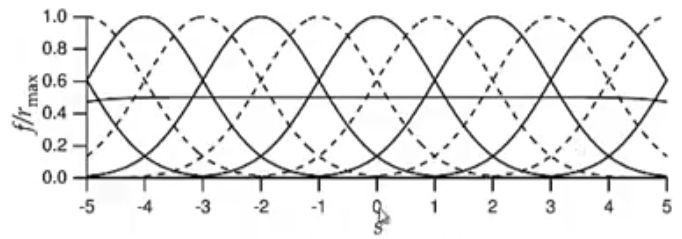
\includegraphics[width=\textwidth]{decode-stimulus}
\end{figure}

\begin{align*}
	f_a(s) =& r_{max} \exp \Big(-\frac{1}{2}\big[\frac{s-s_a}{\sigma_a}\big]^2\Big)\text{, assume good coverage} \numberthis \label{eq:gauss}\\
	\sum_{1}^{N} f_a(s) =& const \numberthis \label{eq:good:coverage}
\end{align*}

So firing rate doesn't depend on stimulus

From assumption \ref{item:poisson}, spikes are produced randomly and independently in each time bin with probability
\begin{align*}
	P_T[k] =& \frac{(rT)^k \exp (-rT)}{k!}\\
	P_T[r_a\vert s] =& \frac{(f_a(s)T)^{r_aT} \exp (-f_a(s)T)}{r_aT!}\\
	P[\vec{r}\vert s] =& \prod_{a=1}^{N}P_r[a\vert s]\\
	=& \prod_{a=1}^{N} \frac{(f_a(s)T)^{r_aT} \exp (-f_a(s)T)}{r_aT!}
\end{align*}

We want the \gls{gls:mlm} for $s$.
\begin{align*}
	\ln P[\vec{r}\vert s] =& \sum_{a=1}^{N} \big[r_aT \ln (f_a(s)T) -f_a(s)T - \ln (r_aT!) \big] \text{, so we need}\\
	\partial_s \ln P[\vec{r}\vert s] =& 0	\\
	\partial_s \ln P[\vec{r}\vert s] = & \partial_a \sum_{a=1}^{N}  r_aT \ln (f_a(s)T) -\underbrace{\partial_a \sum_{a=1}^{N} f_a(s)T}_{=0 \text { from ]\eqref{eq:good:coverage}}} - \underbrace{\partial_a \sum_{a=1}^{N} \ln (r_aT!)}_{=0} 
\end{align*}
Hence the \gls{gls:mlm} is given by:
\begin{align*}
	T \partial_a \sum_{a=1}^{N} r_a  \ln (f_a(s)T) =& 0\\
	 \sum_{a=1}^{N} r_a  \partial_a \ln (f_a(s)T) =& 0\\
	 \sum_{a=1}^{N} r_a  \frac{\partial_a  (f_a(s)\cancel{T})}{(f_a(s)\cancel{T})} =& 0\\
	 \sum_{a=1}^{N} r_a  \frac{\partial_a  f_a(s^*)}{f_a(s^*)} =& 0 \numberthis \label{eq:ml:example}
\end{align*}

\begin{align*}
	\partial_a  f_a(s) =& \partial_a r_{max} \exp \Big(-\frac{1}{2}\big[\frac{s-s_a}{\sigma_a}\big]^2\Big)\\
	=&r_{max}\big[-\frac{1}{\cancel{2}} \frac{\cancel{2}(s-s_a)}{\sigma_a^2}\big] \exp \Big(-\frac{1}{2}\big[\frac{s-s_a}{\sigma_a}\big]^2\Big)\\
	=& \frac{\cancel{2}(s-s_a)}{\sigma_a^2} f_a(s) \text{, so \eqref{eq:ml:example} becomes}
\end{align*}
\begin{align*}
	\sum_{a=1}^{N} r_a  \frac{(s^*-s_a)}{\sigma_a^2} =& 0\\
	s^*  =& \frac{\sum_{a=1}^{N}   \frac{s_a r_a}{\sigma_a^2}}{\sum_{a=1}^{N} \frac{ r_a }{\sigma_a^2}}	\\
	=& \frac{\sum_{a=1}^{N}   p_a s_a r_a}{\sum_{a=1}^{N} p_a r_a} \text{, where the precision $p_a=\sigma_a^{-2}$}\\
	=& \frac{\sum_{a=1}^{N}   s_a r_a}{\sum_{a=1}^{N} r_a} \text{, if all the $s_a$ are equal}
\end{align*}
\subsection{Reading Minds - Stimulus Reconstruction}
We want an estimator, $S_{Bayes}$ that gives the "best" estimate of $s$ given $r$.



\appendix

\printglossaries

\end{document}
